\documentclass[twocolumn]{article}
\usepackage{usenix-2020-09}
\usepackage{biblatex}
\usepackage{inconsolata}
\usepackage{bookmark}
\usepackage{minted}
\usepackage[font=small,skip=2pt]{caption}
\usepackage{xcolor}
\usepackage{graphicx}
\usepackage{float}
\hypersetup{pageanchor=true}
\bibliography{ref}
\definecolor{bg}{rgb}{0.97,0.97,0.97}

\begin{document}
\date{}
\title{\Large \bf AMD Confidential Computing Technologies Evaluation Report}
\author{{\rm Roberto Castellotti}\\TU Munich}
\maketitle

\begin{abstract}
We report a preliminary performance evaluation of AMD SEV (Secure Environment Virtualization) technologies.
We are running virtual machines using QEMU/KVM as Hypervisor on a powerful machine we control.
Details about our environment can be found in section \ref{sec:environment}.

Confidential Computing technologies may be predominant in the future, as more and more customers with sensitive computing workloads move their code from on-premise hardware to public cloud vendors. Being able to identify the performance bottlenecks may be crucial. After thoroughly explaining how the technologies introduced by AMD work we run some benchmarks to measure the impact these have on micro-benchmarks and traditional workloads such as compilation of popular open-source projects.
\end{abstract}

\section{Introduction}

\textit{Confidential Computing} is a topic that started to become relevant in the last years. In the last two decades the way software is shipped to production changed radically, the majority of code deployed nowadays is hosted by cloud providers (Google Cloud Platform, Amazon Web Services, Microsoft Azure, etc.) while some code is still run on-premise for privacy/safety reasons. Confidential Computing aims to provide a safe environment for developers to run highly sensitive code on machines they don't own. 

It is logic customers want to be sure no one can access their disks, memory or CPU registers, neither other customers running virtual machines on the same hardware, nor whoever is controlling the hypervisor, be it  the cloud vendor  or, in worst case scenarios, malign actors who compromised the physical machines. Encryption at rest, designed to prevent the attacker from accessing the unencrypted data by ensuring the data is encrypted when on disk \cite{azure-enc}, has been around for a long time, and is currently supported by all major providers \cite{aws-enc}, \cite{gcp-enc}, \cite{azure-enc} but leaves a few components used in daily computing unencrypted, namely RAM and CPU registers. To tackle this issue major chip producers started to develop technologies to enable \textit{Confidential computing}, namely \textit{AMD Secure Encrypted Virtualization (SEV)} \cite{memory-encryption}, \textit{Intel Trusted Domain Extensions (TDX)} \cite{tdx} and \textit{Arm Confidential Compute Architecture (CCA) \cite{cca}}. In this article we will focus on summarizing the AMD tecnhlogies before we run some measurements to evaluate the impact of Confidential Computing technlogies.

\section{Background}
\subsection{AMD Secure Memory Encryption (SME)}

\textit{AMD Secure Memory Encryption (SME)} is the basic building block for the more sophisticated technologies we' ll cover later, so it is imperative we understand how it works. In a machine with \textit{SME} enabled memory operations are performed via dedicated hardware, in fact, an entirely different chip on die. AMD EPYC™ processors introduced two hardware security components:

\begin{itemize}
    \item a \textit{AES-128 hardware encryption engine} embedded in memory controller,a chip whose job is to make sure data transferred to and from the main memory is encrypted during write operations and decrypted during read operations. See Figure \ref{fig:memory-encryption-fig} to better understand how data is managed when \textit{SME} is used. This memory controller is inside the EPYC SOC, memory lines leaving the SOC are always encrypted
    \item the \textit{AMD Secure Processor}, a small processor providing cryptographic functionality to perform secure key generation and key management
\end{itemize}

\begin{figure}
    \centering
    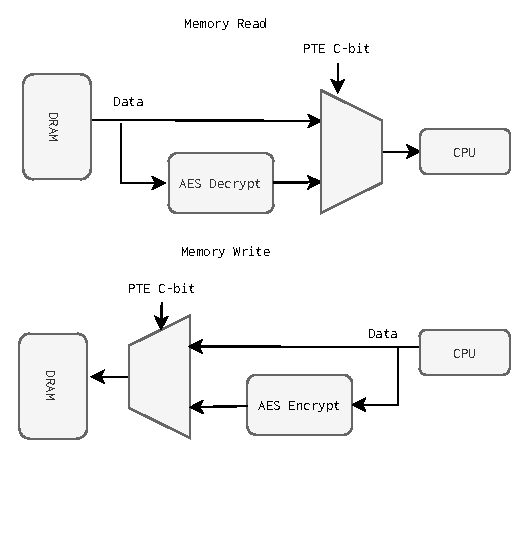
\includegraphics[scale=0.9]{img/read-write.pdf}
    \caption{Memory Encryption Behavior, from \cite{memory-encryption}}
    \label{fig:memory-encryption-fig}
\end{figure}

The AES engine needs a key to work with, this is generated securely by the \textit{AMD Secure-Processor (SMD-SP)}, a 32 bit micro-controller not accessible by software running on the main CPU, furthermore \textit{SME} does not require software running on main CPU to participate in Key Management making the enclave even more secure by reducing the attack surface.

The \textit{C-bit} is a bit present in any memory page and indicates whether the current page is to be encrypted, it can be retrieved together with some additional information by running the \texttt{cpuid} command to inspect leaf \texttt{0x8000001F}, as specified by AMD Reference Manual \cite{architecture-reference}:

\begin{minted}[bgcolor=bg,fontsize=\footnotesize]{bash}
$ cpuid -1 -l 0x8000001F
CPU:
AMD Secure Encryption (0x8000001f):
    SME: secure memory encryption support    = true
    SEV: secure encrypted virtualize support = true
    VM page flush MSR support                = true
    SEV-ES: SEV encrypted state support      = true
    SEV-SNP: SEV secure nested paging        = true
    VMPL: VM permission levels               = true
    Secure TSC supported                     = true
    virtual TSC_AUX supported                = false
    hardware cache coher across enc domains  = true
    SEV guest exec only from 64-bit host     = true
    restricted injection                     = true
    alternate injection                      = true
    full debug state swap for SEV-ES guests  = true
    disallowing IBS use by host              = true
    VTE: SEV virtual transparent encryption  = true
    VMSA register protection                 = true
    encryption bit position in PTE           = 0x33 (51)
    physical address space width reduction   = 0x5 (5)    
    number of VM permission levels           = 0x4 (4)
    number of SEV-enabled guests supported   = 0x1fd (509)
    minimum SEV guest ASID                   = 0x80 (128)
\end{minted}

We can see SME, SEV, SEV-ES and SEV-SNP are enabled, and we can see the \textit{C-bit} on our machine is 51.

SME is a very powerful mechanism to provide memory encryption, but it requires support from the Operating System/Hypervisor, \textit{Transparent SME (TSME)} is a solution to encrypt every memory page regardless of the \textit{C-bit}, as the name suggests this technology provides encryption without further modification to OS/HV, this may be crucial because it means both Operating System developers and Hypervisor developers don't have to implement and mantain additional code and older operating systems can be run in a protected way with TSME.

We now switch our focus to \textit{AMD SEV}, a technology powered by \textit{AMD SME} to enables Confidential Computing for Virtual Machines.

\subsection{AMD Secure Encrypted Virtualization (SEV)}

\textit{AMD SEV} is an attempt to make virtual machines more secure to use by encrypting data to and from a virtual machine, and enables a new security model protecting code from higher privileged resources, such as hypervisors or some privileged code running on the physical machine hosting the virtual machines. In this context, as mentioned before, we should never trust the Hypervisor since it may be compromised or acting maliciously by default.

\begin{figure}
    \centering
    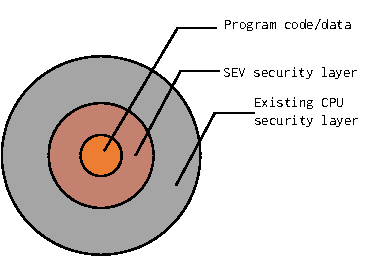
\includegraphics[scale=0.9]{img/security-layers.pdf}
    \caption{SEV security layers, from \cite{memory-encryption}}
\end{figure}

SEV is an extension to the AMD-V architecture, when it is enabled virtual machines tag data with a \textit{VM ASID} (an unique identifier for that specific machine), this tag is used inside the SOC and prevents other virtual machines on the same physical machine to access it, when data leaves the chip we have no such problem because it is encrypted using the previously exchanged AES-128 bit key. The aforementioned expedients provide strong cryptography isolation between VMs run by the same hypervisor and between VMs and the hypervisor by itself. SEV guests can choose which pages to encrypt, this is handled setting the C-bit as mentioned before for SME. Only pages meant for outside communications are considered shared and thus not encrypted. This and other information are discussed more in depth in the introductory whitepaper \cite{memory-encryption}.

\subsection{AMD Secure Encrypted Virtualization-Encrypted State (SEV-ES)}

Up until now we only discussed encryption for memory, but a crucial portion of the system we want to protect are CPU registers, \textit{AMD SEV-ES} encrypts all CPU register contents when a VM stops running. What this means is a malevolent actor won't be able to read CPU's register contents when the machine is shutdown no matter the privilege level he acquired before, CPU registers' state is saved and encrypted when the machine is shutdown.

Protecting CPU register may be a daunting task because sometimes an Hypervisor may need to access VM CPU's register to provide services such as device emulation. These accesses must be protected, ES technology allows the guest VM to decide which registers are encrypted, in the same vein a machine can choose which memory pages are to be encrypted via the C-bit.

\textit{SEV-ES} introduces a single atomic hardware instruction: \texttt{VMRUN}, when this instruction is executed for a guest the CPU loads all registers, when the VM stops running (\texttt{VMEXIT}), register's state is saved automatically to  back to memory. These instructions are atomic because we need to be sure no one can sneak into this process and alter it, ES guarantees in this way it is impossible to leak memory.

Whenever hardware saves registers it encrypts them with the very same AES-128 key we mentioned before, furthermore the CPU computes an integrity-check value and saves it into a memory region not accessible by the CPU, on next \texttt{VMRUN} instruction this will be checked to ensure nobody tried to tamper register's state. For further information about external communication consult the white-paper \cite{protecting-registers} and AMD reference manual chapter 15 \cite{architecture-reference}.

Similarly to \textit{AMD-SEV} \textit{AMD-ES} is completely transparent to application code, guest VM developers and Hypervisors developers are the only one who  need to implement these specific features.

\subsection{AMD Secure Encrypted Virtualization-Secure Nested Paging (SEV-SNP)}

After the introduction of \textit{AMD-SEV} and \textit(AMD-ES) AMD decided to introduce the next generation of SEV called \textit{Secure Nested Paging (SEV-SNP)}, this technology builds on top of the technologies we have seen and extends them further to implement strong memory integrity protection to prevent Hypervisor based attacks, such as \textit{replay attacks} and \textit{memory remapping}, \textit{data corruption} and \textit{memory aliasing}.
Let's now explain what these attacks are before we cover how \textit{SEV-SNP} mitigates them.

\begin{itemize}
    \item a \textit{replay attack} happens when a malicious actor captures a state at a certain moment and modifies memory successfully with those values
    \item \textit{data corruption} attacks happen when even though an attacker, knowing they are not able to read memory, decides to corrupt the memory to trick the machine into unpredicted and possibly dangerous behavior
    \item a \textit{memory aliasing} attack happens when an external actor may map a memory page to multiple physical pages he controls
    \item a \textit{memory remapping} attacks happens wheneverthe intruder maps a page to a different physical page
\end{itemize}

These attacks are a problem because a running program has no notion of memory integrity, it could end up in a state that was not originally considered by the developers and this may lead to huge security issues.

The basic principle of \textit{SEV-SNP} integrity is that if a VM is able to read a private (encrypted) page of memory, it must always read the value it last wrote. What this means is the VM should be able to throw an exception if the memory a process is trying to access was tampered by external actors.

\subsubsection{Threat Model}
In this computing model we consider:
\begin{itemize}
    \item \textit{AMD System-On-Chip (SOC) hardware}, \textit{AMD Secure Processor (AMD-SP)} and the \textbf{VM} as fully trusted, to this extent the VM should enable Full Disk Encryption (FDE) at rest, such as LUKS, major cloud providers have been supporting FDE for long time.
    \item \textbf{BIOS} on the host system, the \textbf{Hypervisor}, \textbf{device drivers} and \textbf{other VMS} as fully untrusted, this means the threat model assumes they are malicious and may conspire to compromise the security of our Confidential Virtual Machine.
\end{itemize}

The way \textit{SEV-SNP} ensures protection against the attacks we mentioned before is by introducing a new data structure, a \textit{Reverse Map Table (RMP)} that tracks owners of memory pages, by having this it is possible to enforce that only the owner of a certain memory page can alter it.

A page can be owned by the VM, the Hypervisor or by the AMD Secure Processor. The RMP is used in conjunction with standard x86 page tables mechanisms to enforce memory restrictions and page access rights.Introducing RMP check for write operations on memory mitigates replay, remapping and data corruption attacks. 

To prevent memory remapping a technique called \textit{Page Validation} is introduced. Inside each RMP entry there is \textit{Validated} bit, pages assigned to guests that have no \textit{validated} bit set are not usable by the Hypervisor, the guest can only use the page after setting the validated bit through a \texttt{PVALIDATE} instruction. The VM will make sure that it is not possible to validate a SPA (system physical address) corresponding to a GPA (Guest Physical Address) more than once.
 
More details are discussed in the introductory white-paper \cite{sev-snp}

We now introduced all the main building blocks of AMD's effort to popularize Confidential Computing, it is now our interest to run some benchmarks to measure if and how these technologies impact performances.

\section{Environment}
\label{sec:environment}
    
We are running our experiments in QEMU/KVM virtual machines, we are assigning 16GB of RAM and 16 vCPUs each, check the table \ref{tab:experiment-environment} to see more details about our hardware and software versions. The code to setup the environment and launch vms is public and can be found at \href{https://github.com/rcastellotti/gr}{https://github.com/rcastellotti/gr}.

\begin{description}
    \item[QEMU] is a generic open source machine emulator and virtualizer \cite{qemu}, we use QEMU together with KVM, the Kernel Virtual machine to virtualize our machines.
    \item[OVMF] is a project maintained by TianoCore \cite{ovmf} aiming to enable UEFI support for virtual machines, it is based on EDK 2, we will use OVMF to generate the executable firmware and the non-volatile variable store, it is important to create a vm-specific copy of \texttt{OVMF\_vars.fd} because the variable store should be private for every virtual machine. UEFI support is mandatory to run a SEV-SNP machine.
\end{description}

\begin{table*}[ht]
    \small
    \centering
    \begin{tabular}{l|l}
        \hline
        Host CPU      & \texttt{AMD EPYC 7713P 64-Cores}                                            \\
        Host Memory   & \texttt{HMAA8GR7AJR4N-XN (Hynix) 3200MHz 64 GB $\times$ 8 (512GB)}          \\
        Host Kernel   & \texttt{6.3.0-rc2 \#1-NixOS SMP PREEMPT\_DYNAMIC (NixOS 23.05)} commit: \href{https://github.com/AMDESE/linux/tree/fea9b785bfa90e015c7d81526e36060da1bf01d1}{\texttt{fea9b78}}            \\
        QEMU          & \texttt{8.0.0 (AMD) (patched)} commit: \href{https://github.com/AMDESE/qemu/tree/a248931547843b9edb0f3b0c7d6d0c76ffdf7659}{\texttt{a248931}}                                             \\
        OVMF          & \texttt{Stable 202211 (patched)} commit: \href{https://github.com/AMDESE/ovmf/commit/6598f62bda4eb884c65d6c0aed7ede64258a41d8}{\texttt{6598f62}}                                     \\
        Guest vCPUs   & \texttt{16}                                                                 \\
        Guest Memory  & \texttt{16GB}                                                               \\
        Guest Kernel  & \texttt{5.19.0-41-generic \#42-Ubuntu SMP PREEMPT\_DYNAMIC (Ubuntu 22.10 )} \\ 
        \hline
    \end{tabular}
    \caption{Experiment Environment}
    \label{tab:experiment-environment}
\end{table*}

\section{Benchmarks}
We expect the aforementioned encryption techniques used in SEV/SEV-ES/SEV-SNP to cause a degradation in performance, especially for memory-intensive workloads, additionally we want to investigate whether this technology slows down CPU intensive workloads and disk opearations. To quantify the price we have to pay to have a more secure virtual environment we are running three distinct kinds of benchmarks: Compilation, Memory Benchmarks and I/O benchmarks. We are using \texttt{rcastellotti/tinyben} \cite{tinyben}, an experimental benchmarking tool aimed to replace the popular Phoronix Test Suite \cite{pts} benchmarking suite.

\begin{description}
    \item[Compilation Benchmarks] We are using compilation as an all-around benchmark because it is a "real world" benchmark. We are compiling some popular open-source projects like \href{https://github.com/godotengine/godot}{Godot Game Engine}, \href{https://git.kernel.org/pub/scm/linux/kernel/git/torvalds/linux.git}{Linux} (defconfig), the entire \href{https://github.com/llvm/llvm-project}{LLVM Project} (using ninja) and measuring how long does it take to complete the compilation process. Check figure \ref{fig:tb-compilation} to see results.
    \item[Memory Benchmarks] To benchmark memory we are using \texttt{ssvb/tinymembench} \cite{tinymembench}, a tool to measure memory throughput and latency, we are mainly interested in bandwidth for the \texttt{MEMCPY} and \texttt{MEMSET} operations. Check figure \ref{fig:tb-tinymembench} to see the results.
    \item[I/O Benchmarks] To measure I/O performance we are running two different benchmarks, first we are performing 2500 sqlite insertions in a table, then we are running redis-benchmark, a tool shipped toghether with redis. We are interested in Requests per Second and latency for the main operations (namely SET and GET). Check figures \ref{fig:tb-misc},\ref{fig:tb-redis} and \ref{fig:tb-redis-latency} to see the results.
\end{description}

As we can see the overhead introduced by the usage of Confidential Computing technology across the three categories of benchmarks is generally mild, and negligible in almost every benchmark, with the exception for LZ4-compression. further investigation tweaking the amount of resources available to each machine is necessary to correctly esteem the exact performance degradation values.

One reason why CPU-intensive workloads are little to no penalized by SEV-SNP is the processor might not be doing much more when executing that kind of workload on a confidential machine, the instructions that really slow down are \texttt{VMEXIT} and \texttt{VMRUN}, we are not issuing any of those during the compilation of a certain program.

\begin{figure}[ht]
    \centering
    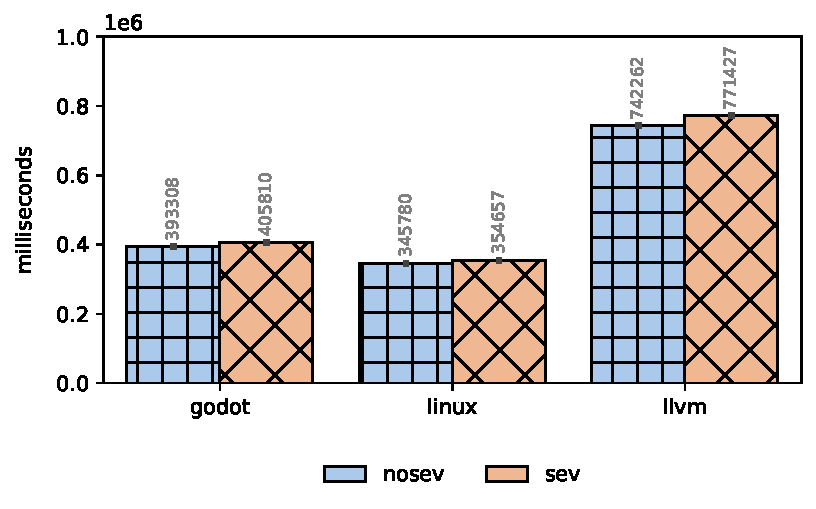
\includegraphics[width=\columnwidth]{img/compilation-benchmark.pdf}
    \caption{Compilation benchmarks, in milliseconds (Lower is Better)}
    \label{fig:tb-compilation}
\end{figure}

\begin{figure}[ht]
    \centering
    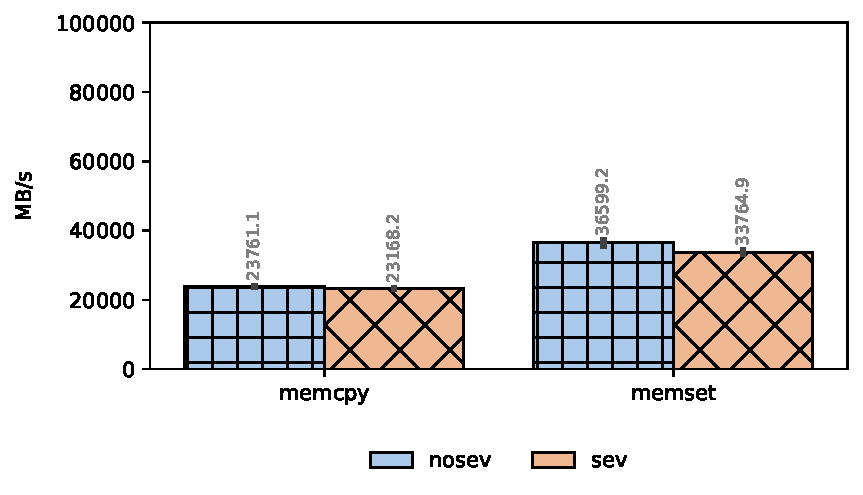
\includegraphics[width=\columnwidth]{img/tinymembenchmark.pdf}
    \caption{tinymembench bandwidth benchmark, \texttt{MEMSET} and \texttt{MEMCPY} (Higher is Better)}
    \label{fig:tb-tinymembench}
\end{figure}

\begin{figure}[ht]
    \centering
    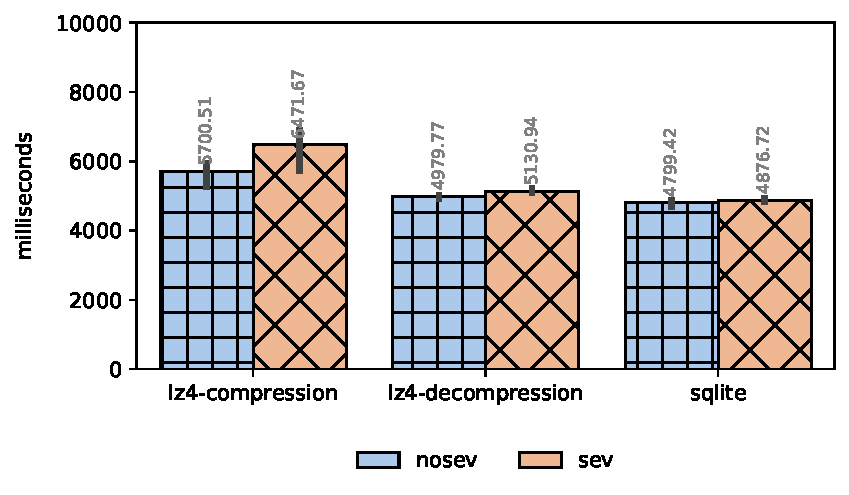
\includegraphics[width=\columnwidth]{img/misc.pdf}
    \caption{Miscellaneous benchmarks, lz4 compression and decompression and Sqlite insertions time to completion (Lower is Better)}
    \label{fig:tb-misc}
\end{figure}

\begin{figure}[ht]
    \centering
    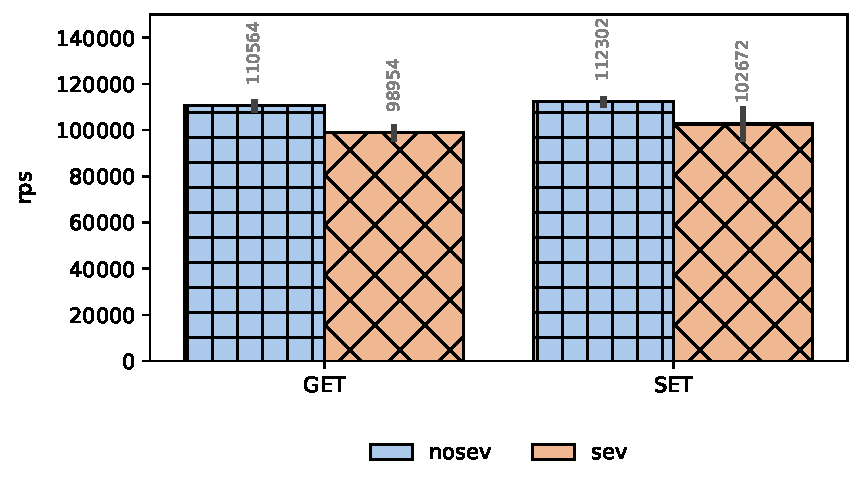
\includegraphics[width=\columnwidth]{img/redis.pdf}
    \caption{Redis-benchmark, SET and GET operations Requests Per Second (Higher is Better)}
    \label{fig:tb-redis}
\end{figure}

\begin{figure}[ht]
    \centering
    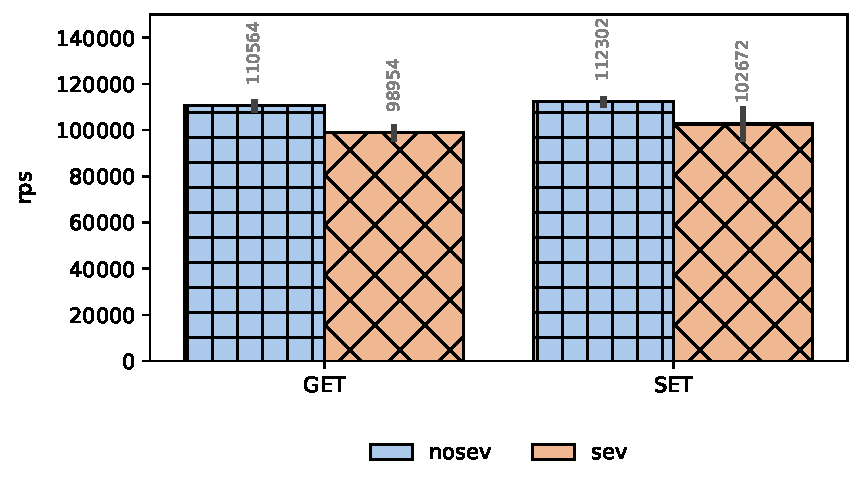
\includegraphics[width=\columnwidth]{img/redis.pdf}
    \caption{Redis-benchmark, SET and GET operations minimum latency(milliseconds) (Lower is Better)}
    \label{fig:tb-redis-latency}
\end{figure}

To investigate storage related operations we ran some additional benchmarks with different storage virtualization techniques, more specifically we tested \textit{virtio-scsi}, \textit{virtio-blk} and \textit{nvme} technologies. Virtio is the main platform for IO virtualization in KVM, essentially it provides a common framework for hypervisors to do IO virtualization.

\begin{description}
    \item[nvme] is the user-space NVMe driver that enables virtual machines to interact with NVMe devices.
    \item[virtio-blk] devices are very simple block devices, the front-end driver reads and writes by appending commands to the virtualization queue so that the back-end driver can process them on the host.
    \item[virtio-scsi] aims to overcome some limitations introduced by virtio-blk, support more devices per guest (one PCI device per disk is not a limiting factor anymore) and supports technologies like multiqueueing while keeping the performances of virtio-blk, additionally virtio-scsi provides a pass-through technology to present physical storage devices directly to guests.\cite{scsi}
\end{description}

We perform some measurements using the FIO \cite{fio} benchmarking tool, we use a similar setup to the one used in \cite{spool} to evaluate: bandwidth, average latency and IOPS, we use the \texttt{--direct=1} flag to use unbuffered I/O. Results are reported in \ref{fig:fio-bw}, \ref{fig:fio-al}, \ref{fig:fio-iops}. We also report the values in tables to better analyze the relative performance variations.

\begin{table*}
    \centering
    \begin{tabular}{l|r|r}
        \hline
        \textbf{benchmark} & \textbf{test cases} & \textbf{FIO Configuration (bs, rw, iodepth, numjobs)} \\
        \hline
        bandwidth          &  read               & (128K, read, 128, 1)                                  \\
        bandwidth          & write               & (128K, write, 128, 1)                                 \\
        IOPS               &  randread           &(4K, randread, 32, 4)                                  \\
        IOPS               & mixread             & (4K, randread 70\%, 32, 4)                            \\
        IOPS               &  mixwrite           & (4K, randwrite 30\%, 32, 4)                           \\
        IOPS               &  randwrite          &  (4K, randwrite, 32, 4 )                              \\
        average latency    &  randwrite          & (4K, randread, 1, 1 )                                 \\
        average latency    &  randwrite          & (4K, randwrite, 1, 1 )                                \\
        average latency    &  read               &(4K, read, 1, 1 )                                      \\
        average latency    &  write	             & (4K, write, 1, 1 )                                    \\
    \end{tabular}
    \caption{FIO benchmarks, from \cite{spool}} 
    \label{tab:fio-benchmarks}
\end{table*}

\begin{figure}
    \centering
    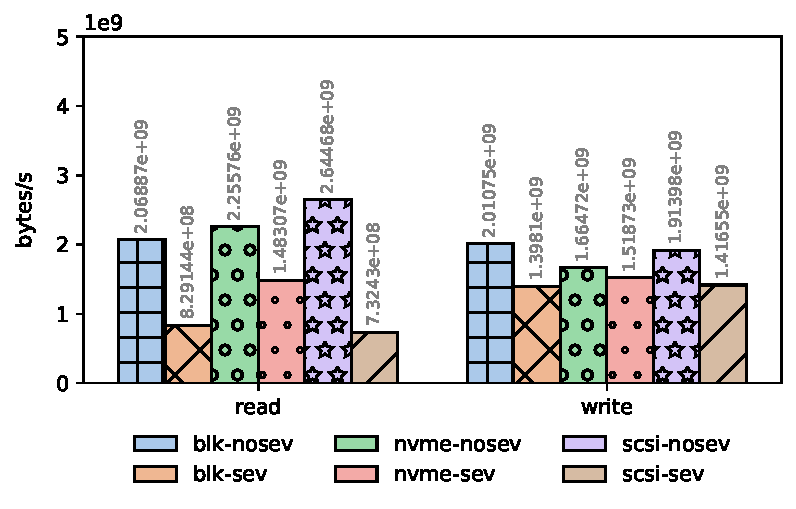
\includegraphics[width=\columnwidth]{img/bw.pdf}
    \caption{Storage Bandwidth Benchmarks (Higher is Better)}
    \label{fig:fio-bw}
\end{figure}

\begin{figure}
    \centering
    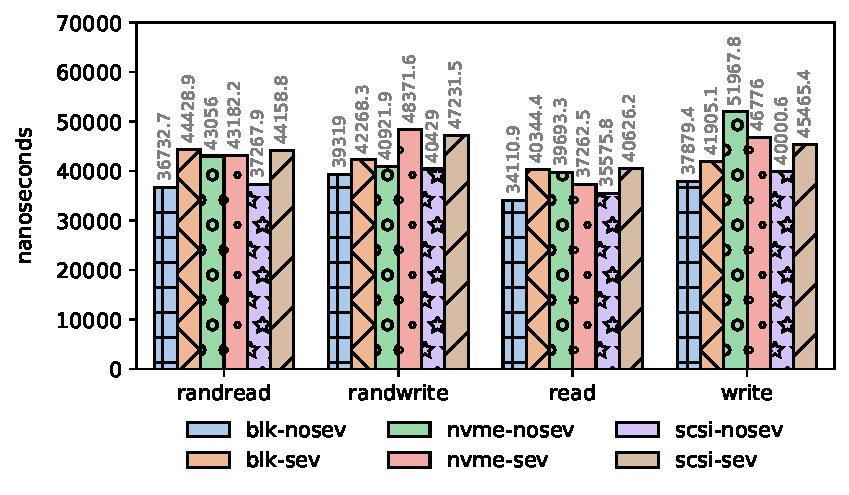
\includegraphics[width=\columnwidth]{img/al.pdf}
    \caption{Average Latency Benchmarks (Lower is Better)}
    \label{fig:fio-al}
\end{figure}

\begin{figure}
    \centering
    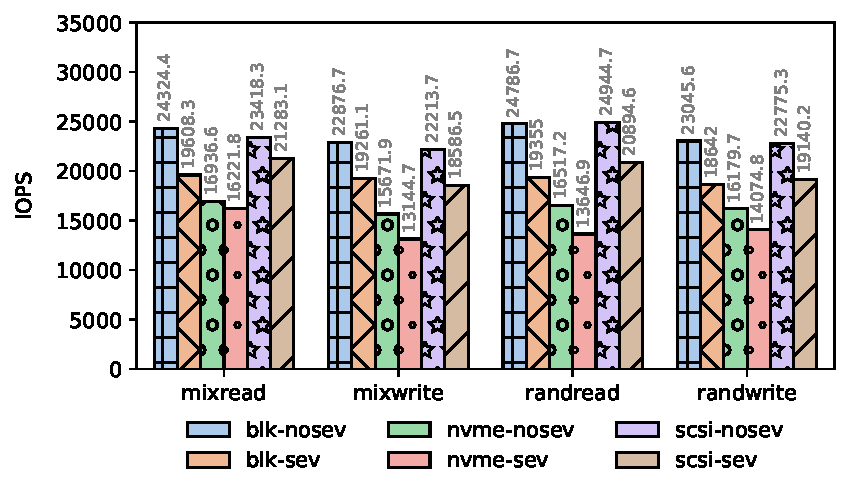
\includegraphics[width=\columnwidth]{img/iops.pdf}
    \caption{IOPS benchmarks (Higher Is Better)}
    \label{fig:fio-iops}
\end{figure}

\begin{table}
    \small
    \begin{tabular}{llllr}
        \hline
        \textbf{mode} & \textbf{storage} & \textbf{nosev} & \textbf{sev} & \textbf{result} \\
        \hline
        read          & blk              & 2068866712     & 829144265    & 0.400772 \\
        read          & nvme             & 2255760134     & 1483068817   & 0.657459 \\
        read          & scsi             & 2644684295     & 732429620    & 0.276944 \\
        write         & blk              & 2010752479     & 1398101333   & 0.695312 \\
        write         & nvme             & 1664716006     & 1518729595   & 0.912306 \\
        write         & scsi             & 1913978295     & 1416545941   & 0.740106 \\
        \hline
    \end{tabular}
    \caption{FIO bandwidth benchmarks results, measured in KB/s,  ratio is the ratio between \textbf{sev} and \textbf{nosev}}
    \label{tab:fio-bw-ratios}
\end{table}

\begin{table}
    \small
    \begin{tabular}{llllr}
        \hline
        \textbf{mode} & \textbf{storage} &  \textbf{nosev} & \textbf{sev} & \textbf{result} \\
        \hline
        mixread       & blk              & 24324.394544    & 19608.347670 & 0.806119        \\
        mixread       & nvme             & 16936.555110    & 16221.782178 & 0.957797        \\
        mixread       & scsi             & 23418.259782    & 21283.104652 & 0.908825        \\
        mixwrite      & blk              & 22876.690811    & 19261.131521 & 0.841954        \\
        mixwrite      & nvme             & 15671.907694    & 13144.662288 & 0.838740        \\
        mixwrite      & scsi             & 22213.710702    & 18586.500284 & 0.836713        \\
        randread      & blk              & 24786.686838    & 19354.991140 & 0.780862        \\
        randread      & nvme             & 16517.169681    & 13646.936332 & 0.826227        \\
        randread      & scsi             & 24944.714055    & 20894.627770 & 0.837637        \\
        randwrite     & blk              & 23045.626374    & 18642.013938 & 0.808918        \\
        randwrite     & nvme             & 16179.730897    & 14074.845638 & 0.869906        \\
        randwrite     & scsi             & 22775.325804    & 19140.186916 & 0.840391        \\
        \hline
    \end{tabular}
    \caption{FIO IOPS benchmarks results, ratio is the ratio between \textbf{sev} and \textbf{nosev}}
    \label{tab:fio-iops-ratios}
\end{table}

\begin{table}
    \small
    \begin{tabular}{lllll}
        \hline
        \textbf{mode}& \textbf{storage} & \textbf{nosev} & \textbf{sev} & \textbf{ratio} \\
        \hline
        randread     & blk              & 36732.676746   & 44428.919037 & 1.209520       \\
        randread     & nvme             & 43056.001194   & 43182.237293 & 1.002932       \\
        randread     & scsi             & 37267.866497   & 44158.765942 & 1.184902       \\
        randwrite    & blk              & 39318.967918   & 42268.305611 & 1.075011       \\
        randwrite    & nvme             & 40921.898750   & 48371.563309 & 1.182046       \\
        randwrite    & scsi             & 40428.971912   & 47231.466854 & 1.168258       \\
        read         & blk              & 34110.888638   & 40344.405910 & 1.182743       \\
        read         & nvme             & 39693.322182   & 37262.537930 & 0.938761       \\
        read         & scsi             & 35575.824402   & 40626.232517 & 1.141962       \\
        write        & blk              & 37879.406013   & 41905.050934 & 1.106275       \\
        write        & nvme             & 51967.809612   & 46775.977871 & 0.900095       \\
        write        & scsi             & 40000.623734   & 45465.357731 & 1.136616       \\
        \hline
    \end{tabular}
    \caption{FIO average latency benchmarks, measured in nanoseconds, ratio is the ratio between \textbf{sev} and \textbf{nosev}}
    \label{tab:fio-al-ratios}
\end{table}

The FIO benchmarks highlight some interesting patterns: bandwidth is severely impacted, especially in read workloads, this might be related to the usage of the aforementioned \textbf{Reverse Map Table}. The number of Input/Output Operations per second
is always lower on the SEV machine, as expected, however the difference is very contained. Average latency is almost always worse on SEV machines, in certain cases it is marginally lower, but we believe this is due to some artifact and is not relevant.

\section{Final Remarks and Conclusion}
Overall, from a first evaluation, it seems SEV/SEV-ES/SEV-SNP tecnhlogies do not introduce a noticeable degradation in performance. The only exception is read bandwidth across all different storage virtualization tecnhniques, further evaluation may be needed to better pinpoint what causes this decrease in performace.
All the code to run virtual machines and benchmarks is public, MIT licensed, except where noted, and available at \href{https://github.com/rcastellotti/gr}{https://github.com/rcastellotti/gr}

\section{Future Work}
Further performance evaluation for SEV/SEV-ES/SEV-SNP confidential virtual machines will include:

\begin{itemize}
    \item repeating micro-benchmarks and FIO benchmarks tweaking machines configuration (vCPUs, RAM, storage virtualization)
    \item analyzing IO performance when using SEV Trusted Input Output \cite{tio}
    \item analyzing whether having multiple SEV machines on the same physical host incurs in a large overhead
    \item analyze performance overhead caused by \texttt{VMRUN} and \texttt{VMEXIT} when SEV-ES is enabled.
    \item investigate unikernels supporting SEV like \href{https://github.com/microsoft/monza}{microsoft/monza}
    \item exploring Confidential Containers \cite{coco} project to identify potential bottlenecks
    \item understand AMD Secure VM Service Module \cite{svsm}, a module to offload sensitive operations onto a privileged guest and see if this leads to a performance improvement
\end{itemize}

    
\printbibliography
\appendix

\section{Appendix}
\subsection{A simple attack to demo Confidential Computing}
Let's demo a very simple attack, first of all we start two machines, \textit{sev} and \textit{nosev}, the former has SEV-SNP enabled, as we can check:

\begin{minted}[bgcolor=bg,fontsize=\footnotesize]{bash}
sev:~$ sudo dmesg | grep SEV
Memory Encryption Features active: AMD SEV SEV-ES SEV-SNP
SEV: Using SNP CPUID table, 31 entries present.
SEV: SNP guest platform device initialized.
\end{minted}

We will write something into a file and cat it in order to load the data in memory

\begin{minted}[bgcolor=bg,fontsize=\footnotesize]{bash}
sev:~$ echo "hi from SEV!" > sev.txt
sev:~$ cat sev.txt
hi from SEV!
\end{minted}

\begin{minted}[bgcolor=bg,fontsize=\footnotesize]{bash}
nosev:~$ echo "hi from NOSEV!" > nosev.txt
nosev:~$ cat nosev.txt
hi from NOSEV!
\end{minted}

Now we can dump the memory for the processes using \texttt{gcore}

\begin{minted}[bgcolor=bg,fontsize=\footnotesize]{bash}
h:~$ sudo gcore -o mem-dump <SEV_PID>
h:~$ grep -rnw mem-dump.<SEV_PID> -e "hi from SEV!"
h:~$
\end{minted}

\begin{minted}[bgcolor=bg,fontsize=\footnotesize]{bash}
h:~$ sudo gcore -o mem-dump <NOSEV_PID>
h:~$ grep -rnw mem-dump.<NOSEV_PID> -e "hi from NOSEV!"
grep: mem-dump.<NOSEV_PID>: binary file matches
\end{minted}

From the host machine we are able to see nosev's machine memory while this is not possible with SEV enabled.

\end{document}